\chapter{Algorithmen}\label{ch:algorithmen}
Verschiedene Theorien/Strategien von Speicher und Ladesysteme ausarbeiten und Zeiten messen (Mit Java und JSON hauptsächlich). Verschiedene Spielarten und Speichersysteme für diese ausarbeiten (Chunk Systeme machen vielleicht nicht überall Sinn, aber allgemein Daten aufteilen müsste gut sein)
%--------------------------------------------------------------------------
%--------------------------------------------------------------------------




%--------------------------------------------------------------------------
%--------------------------------------------------------------------------
\section{Speichersysteme}\label{sect:speichersysteme}
Theorie/Strategien von Speichersystemen und Bezug auf Arten von Videospiel-Daten.

Wichtiger unterschied zwischen ersten Speichern und das Speichern danach. Beim ersten Mal muss die Grundstruktur aufgebaut werden und auch mehr gespeichert werden.
%--------------------------------------------------------------------------


%--------------------------------------------------------------------------
\subsection{Daten in Videospielen}
Um sich weiter mit Speicher- und Ladesystemen auseinander zu setzen, muss erst einmal definiert werden, welche Arten von Daten es in Videospielen gibt. Allgemein können die Daten in zwei Kategorien unterteilt werden. Ein Videospiel hat \textit{statische} und \textit{dynamische} Daten.

\textit{Statische Daten} sind wie der Name es schon sagt Daten, die sich nicht mehr verändern. Statische Daten eines Spieles können zum Beispiel die ganzen Grafikdaten und audiotechnischen Daten sein. Spiele haben fast immer Charaktere, Texturen, Musik oder Soundeffekte die einmal erstellt werden und danach unverändert im Spiel geladen werden. Bei vielen Videospielen gibt es auch Level- oder Kartendaten. Wenn diese sich nie während des Spieles verändern und fest definiert sind, sind diese ebenfalls eine Art von statischen Spieldaten. \wichtig{Updaten von statischen Daten erwähnen (Paper einbeziehen)}

\textit{Dynamische Daten} dagegen sind auch wie es der Name verrät Daten, die sich ständig verändern können. Hierbei handelt es sich oft um den Spielstand eines erstellten Spieles. Dazu gehören dann zum Beispiel die Position des Spielers, seine Rotation, seine aktuelle Geschwindigkeit oder sein Inventar. Alles Daten, die sich andauernd während des Spielens verändern können. Zu den dynamischen Daten können auch Benutzerdaten gehören. Bei einigen Spielen wird ein Benutzername mit Passwort und Avatar benötigt. Dies sind auch Daten, die sich gelegentlich verändern können.

Der Fokus dieser Arbeit liegt bei dynamischen Daten, genauer gesagt wie der Spielstand eines Spieles effizient gespeichert und geladen werden kann. Für Dynamische Daten gibt es viel mehr Speicherprozesse während der Laufzeit des Videospiels, was das effiziente Speichern herausfordernder macht. Da Benutzerdaten recht selten sich verändern, stehen diese auch nicht im Schwerpunkt der Arbeit.  
%--------------------------------------------------------------------------


%--------------------------------------------------------------------------
\subsection{Spielphasen}
Um zu verstehen, wann ein Spielstand gespeichert oder geladen werden muss, muss erst einmal analysiert werden, welche Phasen ein Videospiel allgemein hat.

\begin{figure}[htp]
    \centering
    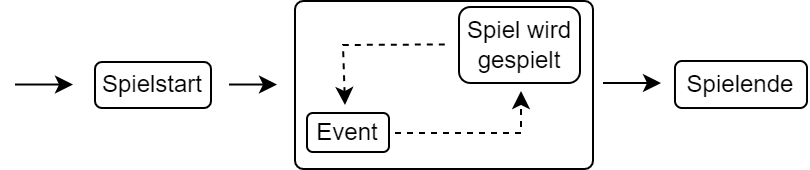
\includegraphics[width=0.8\textwidth]{images/Spielphasen.png}
    \caption{Phasen eines Spieles}
    \label{fig:spielphasen}
\end{figure}

In der Abbildung \ref{fig:spielphasen} ist zu erkennen, wie der Ablauf einer generellen Spielphase in Videospielen gestaltet ist. Der Prozess beginnt mit dem Spielstart, bei dem der Benutzer die Wahl zwischen dem Erstellen eines neuen Spiels oder dem Laden eines bereits vorhandenen Spielstands treffen muss. Sobald diese Eröffnungsphase abgeschlossen ist, wird die Hauptphase erreicht. Die Dauer dieser Phase hängt von der Spieldauer ab, da hier der Benutzer aktiv ins Geschehen eingreift und das Videospiel spielt.

In dieser Spielphase können vielfältige Ereignisse auftreten, die entweder direkt oder indirekt als Reaktion auf die Aktionen des Spielers entstehen. Die Ereignisse äußern sich in Form von Veränderungen an Spielobjekten, entweder durch Modifikation, Hinzufügung oder Löschung dieser. Beispielsweise kann der Spieler in eine neue Region vorstoßen, wodurch Daten dieser Region geladen und möglicherweise Daten der vorherigen Region gespeichert werden müssen. Das Spielobjekt des eigenen Charakters wurde in diesem Fall verändert, denn es wurde zum Beispiel die Position und Region des Spielers verändert. Vielleicht müssen dann auch neue Gegner erstellt oder stehen gelassene Items der alten Region gelöscht werden. 

Sobald der Spieler sich dazu entscheidet, das Spiel zu beenden, gelangt er zur Phase des Spielendes. Hierbei ist es eventuell erforderlich, Daten zu speichern, bevor das Programm ordnungsgemäß beendet werden kann, oder die Rückkehr zum Hauptbildschirm des Spiels erfolgt. Diese Phase des Spielendes markiert einen Schlusspunkt im aktuellen Spielsitzung. Wenn diese wieder fortgesetzt werden soll, muss der Spielstand, der bei dem letzten Beenden des Spieles erreicht wurde wieder vollständig hergestellt werden. 
%--------------------------------------------------------------------------


%--------------------------------------------------------------------------
\subsection{Delta-basierte Speicherung}
Um die Menge der zu speichernden Daten zu reduzieren, empfiehlt es sich, auf eine delta-basierte Speicherung zurückzugreifen. Bei dieser Methode werden lediglich die Daten gespeichert, die sich seit dem letzten Speichervorgang verändert haben. Insbesondere bei großen Datenmengen entfaltet diese Speichertechnik ihre volle Effektivität, da dann oft nur ein geringer Prozentsatz der Gesamtdatenmenge tatsächlich abgespeichert werden muss und somit der Speicherbedarf stark reduziert wird. Um stets den Überblick darüber zu behalten, welche Veränderungen eingetreten sind, gilt es, auf Ereignisse zu achten, bei denen Modifikationen, Hinzufügungen oder Löschungen von Spielobjekten auftreten.
%--------------------------------------------------------------------------


%--------------------------------------------------------------------------
\subsection{Aufteilung der Daten}
Eine weitere Art um die Datenmenge besser zu organisieren um dann Speicherprozesse zu reduzieren, ist das Aufteilen der Daten. Wenn die ganze Datenmenge in sinnvolle Gruppen unterteilt wurde, ist es nicht notwendig jedes mal die ganze Datenmenge zu durchlaufen. Stattdessen kann sich immer nur eine bestimmte Gruppe vorgenommen werden.

Eine sehr weit verbreitete Art der Aufteilung von Spieldaten sind \textit{Chunks}. Chunks haben bei Videospielen meist eine feste Position und sind alle gleich groß. Daten werden dann abhängig von deren Position zu dem entsprechenden Chunk zugeteilt. Vorteilhaft an dieser Herangehensweise ist, dass recht einfach und schnell gefiltert werden kann, welche Daten bei dem aktuellen Spielstand relevant sind. Beim Speichern und Laden können dann nur Chunks in der Nähe des Spielers betrachtet werden. Außerdem können Spielwelten mit dieser Struktur theoretisch unendlich sein, die Größe muss nicht fest gesetzt sein. Es gibt auch Variationen von Chunk-Systemen. Es kann zum Beispiel entschieden werden, ob ein \textit{statisches} oder \textit{dynamisches Chunk-System} verwendet werden soll. Bei einem \textit{statischen Chunk-System} wird die Chunkgröße fest auf einen Wert definiert und wird sich auch nie verändern. Bei einem \textit{dynamischen Chunk-System} passen sich die Chunkgrößen an, je nach Menge der Daten in einem Chunk. Wenn zu viele Daten in einem Chunk sind, werden weitere Chunks erstellt, um die Daten des ursprünglichen Chunks auf diese aufzuteilen. Die Abbildung \ref{fig:chunkSplitting} zeigt ein Beispielszenario, wo in einem Chunk zu viele Charaktere sind und dieser dann in vier gleich große Chunks aufgeteilt wird. Wenn zu wenig Daten in einem Chunk sind, dann werden benachbarte Chunks wieder vereinigt, um sich die Daten zu teilen. Die Abbildung \ref{fig:chunkJoining} demonstriert den Fall, dass vier benachbarte Chunks zu wenig Inhalt haben und deshalb zu einen einzelnen Chunk vereint werden. Diese Variation des Chunk-Systems ist gerade dann sinnvoll, wenn sich die Datenmenge stetig und stark verändern kann. \wichtig{Nur nötig, wenn theoretisch unendlich viele Objekte in einem Chunk existieren können. }
\wichtig{Mehr Quellen, aus Google Scholar}

\begin{figure}[htp]
    \centering
    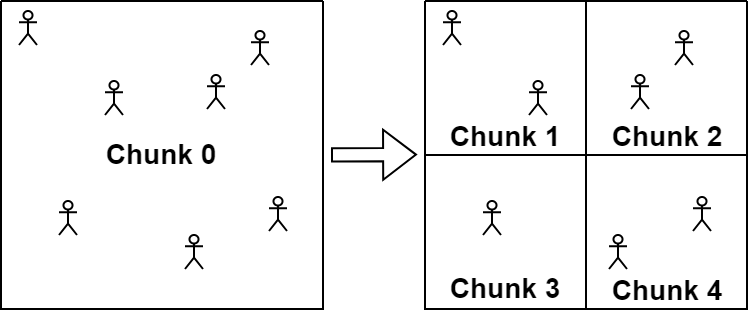
\includegraphics[width=0.6\textwidth]{images/chunkSplitting.png}
    \caption{Vollen Chunk auf kleinere aufteilen}
    \label{fig:chunkSplitting}
\end{figure}

\begin{figure}[htp]
    \centering
    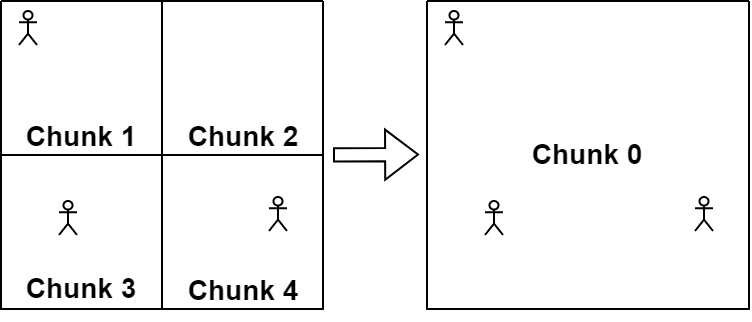
\includegraphics[width=0.6\textwidth]{images/chunkJoining.png}
    \caption{Leere Chunks vereinigen}
    \label{fig:chunkJoining}
\end{figure}

Wenn die Spielwelt aus statischen Elementen wie Level oder Karten besteht, dann können die Daten auch nach Szenen oder Räumen aufgeteilt werden. Es können dann immer nur die Szenen oder Räume gespeichert oder geladen werden, in dem der Spieler sich momentan befindet. Falls die Szenen oder Räume zu groß werden, können diese auch in Sektoren oder Chunks aufgeteilt werden, damit nicht zu viele Daten durchlaufen werden müssen.    
%--------------------------------------------------------------------------


%--------------------------------------------------------------------------
\subsection{Serialisieren}
%\url{https://en.wikipedia.org/wiki/Comparison_of_data-serialization_formats}

\textit{Serialisierung} ist der Prozess, bei dem ein Objekt zu eine Ansammlungen von Bytes umgewandelt wird oder der Zustand eines Objekts in ein Medium abgespeichert wird, um es später wiederherzustellen oder zu übertragen, wobei die Datenstruktur und der Inhalt des Objekts in einer für die Speicherung oder Übertragung geeigneten Form kodiert werden. \textit{Deserialisierung} ist der Gegenprozess von Serialisierung, der den zuvor serialisierten Zustand wieder in das ursprüngliche Objektformat zurückführt, indem die kodierten Daten aus dem Medium extrahiert werden, die ursprüngliche Datenstruktur rekonstruiert und folglich das Objekt in seinen initialien Zustand zurückversetzt.\cite{codeguruWorkingWith}

\subsubsection{JSON}
Eine sehr beliebte Möglichkeit Objekte auf Medien abzuspeichern ist im JSON-Format\footnote{JavaScript Object Notation \wichtig{Ins Abkürzungsverzeichnis?}}. JSON ist eine Codierung von Daten, die für Menschen lesbar ist und wurde anfang der 2000er Jahre erfunden. JSON Objekte sind Ansammlungen von Werten, denen jeweils ein Schlüssel in der Form eines String\footnote{Zeichenketten}-Wertes zugeordnet wird. Unterstützte Datentypen sind String, Boolean, Number, Array, Object und null. JSON wird häufig für APIs, Konfigurations-Dateien und als Datenbank-Speicher verwendet. Aber es kann auch dazu verwendet werden, dass der Zustand eines Objektes in lokalen Dateien abgespeichert wird.\cite{mongodbJSONBSON} 
In dem Code aus \ref{lst:jsonExp} ist zu sehen, wie ein Objekt in dem JSON-Format abgespeichert werden kann. Das entsprechende Klassendiagramm des zu speichernden Objektes ist in der Abbildung \ref{fig:monsterBspKlasse} zu sehen. Das Objekt "position" besteht aus den Variablen x und y, die den Typ Number speichern und das "effects" Array ist ein String-Array. 

\begin{listing}[htp]
    \begin{minted}{javascript}
        {
            "id": 1,
            "name": "Vampir",
            "position": {
                "x": 0.15,
                "y": 2.34
            },
            "effects": [
                "giftig", 
                "frost"
            ]
        }
    \end{minted}
    \caption{Beispiel für ein JSON-Objekt}
    \label{lst:jsonExp}
\end{listing}

\begin{figure}[htp]
    \centering
    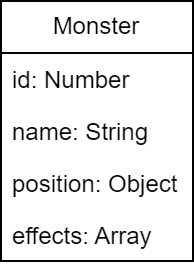
\includegraphics[width=0.18\textwidth]{images/MonsterBspKlasse.png}
    \caption{Klassendiagramm des Beispiel JSON-Objektes aus \ref{lst:jsonExp}}
    \label{fig:monsterBspKlasse}
\end{figure}

Wenn sich für JSON entschieden wurde, gibt es drei Arten die Daten zu verarbeiten. Die erste ist mit einer \textit{Streaming API}, mit der man direkt JSON-Objekte mit Schlüsseln und Werten erstellen kann oder direkt auf Schlüsselwerte von JSON-Objekten zugreifen kann über den entsprechneden Schlüssel. In dem Pseudocode \ref{lst:streamingApiBsp} ist zu sehen, wie mit einer Streaming API das JSON-Objekt aus \ref{lst:jsonExp} erstellt werden kann. Die letzten drei Zeilen sollen ein Zugriff auf Werte des JSON-Objektes darstellen.\cite{tutorialspointJacksonStreaming} Das \textit{Tree Model} dagegen arbeitet mit einem JSON Document, welches in dem Arbeitsspeicher als Baumstruktur gespeichert wird, wodurch das aktualisieren von Daten sehr schnell abläuft. Diese Baumstruktur kann dann als JSON-String in einer lokalen Datei abgespeichert werden. Zu letzt gibt es noch das \textit{Data Binding}, welches die Objekte direkt zu JSON serialisiert und umgekehrt deserialisiert. In dem Pseudocode \ref{lst:dataBindingBsp} ist zu sehen, wie ein neu erstelltes Objekt direkt als JSON-Objekt in eine Datei gespeichert wird. Das Objekt ist aus der Monster-Klasse der Abbildung \ref{fig:monsterBspKlasse}. Danach wird das Objekt mit den Werten eines JSON-Objektes einer anderen Datei gesetzt.\cite{tutorialspointJacksonData}\cite{tutorialspointJacksonOverview}

\begin{listing}[htp]
    \begin{minted}{java} 
        writeStartObject()
        writeField("id", 1)
        writeField("name", "Vampir")
        writeField("name", "Vampir")
        writeFieldName("position")
        writeStartObject()
        writeField("x",  0.15) 
        writeField("y",  2.34) 
        writeEndObject()
        writeFieldName("effects")
        writeStartArray()
        write("giftig") 
        write("frost")
        writeEndArray()

        get("id")
        get("position").get("x")
        get("effects")[0]
    \end{minted}
    \caption{Psuedocode Beispiel für eine Streaming API}
    \label{lst:streamingApiBsp}
\end{listing}

\begin{listing}[htp]
    \begin{minted}{java} 
        Monster monster = new Monster()
        monster.setID(1)
        monster.setName("Vampir")
        monster.setPosition(new Position(0.15, 2.34))
        monster.setEffects(new String[]{"giftig", "frost"})
        toJSON("data1.json"monster)

        monster = toObject("data2.json")
    \end{minted}
    \caption{Psuedocode Beispiel für Data Binding}
    \label{lst:dataBindingBsp}
\end{listing}

BSON:
\begin{itemize}
    \item Binary JSON
    \item Kodiert JSON-Typen und speichert deren Länge (wodurch das Durchqueren der Daten schneller als bei JSON läuft)
    \item Nicht menschlich lesbar wie JSON
    \item Unterstützt mehr Typen
\end{itemize}
\url{https://www.mongodb.com/json-and-bson}

\begin{listing}[htp]
    \begin{minted}{javascript}
        {"hello": "world"}
    \end{minted}
    \caption{Weiteres Beispiel eines JSON-Objektes}
    \label{lst:bsonJsonObj}
\end{listing} 

\begin{listing}[htp]
    \begin{minted}{javascript} 
        \x16\x00\x00\x00           
        \x02                      
        hello\x00                  
        \x06\x00\x00\x00world\x00  
        \x00                       
    \end{minted}
    \caption{Beispiel für ein BSON-Objekt}
    \label{lst:bsonExp}
\end{listing}

Das JSON-Objekt \ref{lst:bsonJsonObj} wäre äquivalent zu dem BSON-Objekt \ref{lst:bsonExp}. Die Zeilen bedeuten folgendes:
\begin{enumerate}
    \item Gesamt Dokument Größe
    \item 0x02 = Typ String
    \item Field-Namen
    \item Field-Werte
    \item 0x00 = Ende des Objekts
\end{enumerate}
\url{https://www.mongodb.com/json-and-bson} % 28.7.2023

JSONH: (\url{https://stackoverflow.com/questions/11160941/is-it-worth-the-effort-to-try-to-reduce-json-size})



Binäre Serialisierung:
\begin{itemize}
    \item Konvertierung von Objekt zu Stream von Bytes
    \item Nicht leserlich für Menschen
\end{itemize}
\url{https://learn.microsoft.com/en-us/previous-versions/dotnet/fundamentals/serialization/binary/binary-serialization}
%--------------------------------------------------------------------------


%--------------------------------------------------------------------------
\subsection{Komprimierung der Daten}
Zippen der Daten:
\begin{itemize}
    \item Viel zippen vs. kleine Dateien (Kleine Chunks)
    \item Bringt lokales Zippen überhaupt was oder nur wenn man mit Server arbeitet?
\end{itemize}

Weitere Ideen:
\begin{itemize}
    \item Kürzere property Namen
    \item Null Werte ausschließen
    \item Vectoren in einem String (z.B. "1,2,3" für x=1, y=2, z=3)
\end{itemize}
%--------------------------------------------------------------------------


%--------------------------------------------------------------------------
\subsection{Schreibprozesse reduzieren}
Das Schreiben in den normalen Speicher ist zeitintensiv. Deshalb sollte möglichst wenig Daten auf die Festplatte geschrieben werden. Eine Möglichkeit ist es, die Veränderungen über eine Liste im Arbeitsspeicher zu speichern und bei Programmterminierung diese Liste abzuspeichern. Dies ist aber riskant, da Daten verloren gegangen werden können bei frühzeitigen Löschen. Alternativ kann man diese Liste auf dem Festplattenspeicher führen und beim Laden des Spieles abarbeiten und dann leeren.
%--------------------------------------------------------------------------
%--------------------------------------------------------------------------




%--------------------------------------------------------------------------
%--------------------------------------------------------------------------
\section{Ladesysteme}\label{sect:ladesysteme}
Theorie vom Laden der Spieldaten
%--------------------------------------------------------------------------


%--------------------------------------------------------------------------
\subsection{Nearby Loading} \label{ssect:nearbLoading}
Nur die Daten laden, die in der Nähe vom Spieler sind (über Render-Distance). Ein Chunk-System (oder allgemein gute Aufteilung der Daten) dafür sehr vorteilhaft für effizienteres Laden, statt durch alle Elemente immer zu iterieren.
%--------------------------------------------------------------------------


%--------------------------------------------------------------------------
\subsection{Lazy Loading}
Prozedulares Laden der Daten (nicht alles auf einmal laden, sondern erst mal nur das nötigste und dann Stück für Stück den Rest nachladen). 
%--------------------------------------------------------------------------


%--------------------------------------------------------------------------
\subsection{Leseprozesse reduzieren}
\wichtig{Gibt vielleicht hier was zu schreiben}
%--------------------------------------------------------------------------
%--------------------------------------------------------------------------




%--------------------------------------------------------------------------
%--------------------------------------------------------------------------
\section{Strategien}
Aus den Strategien der vorherigen sections verschiedene Speicher- und Ladesysteme aufstellen und deren Effizienz auswerten.

\subsection{Allgemeines Speicher- und Ladesystem}
Allgemeines Speicher- und Ladesystems (manche Schritte optional)
\begin{figure}[htp]
    \centering
    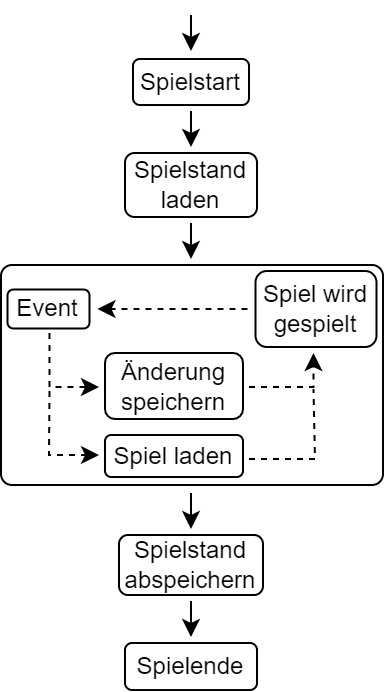
\includegraphics[width=0.36\textwidth]{images/Speichersystem.png}
    \caption{Phasen eines allgemeinen Speicher- und Ladesystems}
    \label{fig:speicherphasen}
\end{figure}

\begin{itemize}
    \item Spielstand laden kann alles auf einmal oder nur teile geladen werden (siehe mehr im Kapitel \ref{sect:ladesysteme})
    \item Je nach Speichersystem müssen hier teilweise noch die gespeicherten Daten überarbeitet werden
    \item Je nach Speichersystem können die Events die in "Änderung speichern" behandelt werden in zwei Kategorien unterteilt werden:
    \begin{enumerate}
        \item Ein Spielobjekt wurde hinzugefügt/geändert
        \item Ein Spielobjekt wurde gelöscht
    \end{enumerate}
    \item Spiel laden nach Events, wenn der Spieler sich z.B. in neuen Bereichen der Map befindet, die noch geladen werden müssen (mehr dazu in \ref{sect:ladesysteme})
    \item Spielstand am Ende abspeichern, vor Spielende optional (je nach Speichersystem notwendig)
\end{itemize}
%--------------------------------------------------------------------------


%--------------------------------------------------------------------------
\subsection{Chunk-basiertes System}
Chunk-basiertes System, welches Daten in Chunks verpackt:
\begin{figure}[htp]
    \centering
    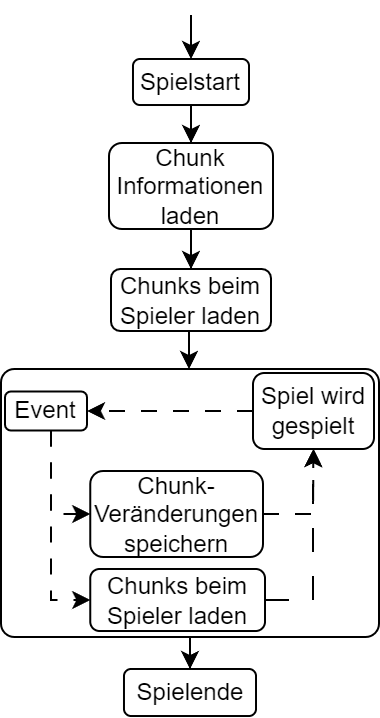
\includegraphics[width=0.36\textwidth]{images/Chunkbasiert.png}
    \caption{Chunk-basiertes System}
    \label{fig:chunkBasedSystem}
\end{figure}

Wobei ein Chunk aus folgenden Variablen besteht:
\begin{figure}[htp]
    \centering
    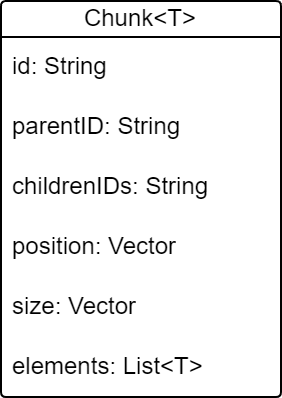
\includegraphics[width=0.28\textwidth]{images/Chunk.png}
    \caption{Chunk Klasse}
    \label{fig:chunkClass}
\end{figure}

\begin{itemize}
    \item Chunks haben Position und Größe
    \item Dynamische oder statische Chunk Größe (Entweder alle Chunks feste Größe, oder sie passen sich an Datenmenge an)
    \item Chunks speichern Objekte, die in deren Bereich sind
    \item ParentID und ChildrenIDs sind optional
\end{itemize}

Informationen zu dem System:

\begin{itemize}
    \item Objekte von Chunks in der Nähe des Spielers laden
    \begin{itemize}
        \item Allgemein werden Objekte eines Chunks erst dann laden, wenn es nötig ist (Z.B. Spieler in der Nähe); sowohl am Anfang, als auch während des Spieles
    \end{itemize}
    \item Chunk Veränderungen speichern bei statischer Chunkgröße:
    \begin{itemize}
        \item Daten zu Chunkinhalt komplett neu speichern bei update/added/removed Objekt Event
    \end{itemize}
    \item Chunk Veränderungen speichern bei dynamischer Chunkgröße:
    \begin{itemize}
        \item Daten zu Chunkinhalt komplett neu speichern bei update/added Objekt Event 
        \item Chunkgröße bei added/removed Objekt Event überprüfen
        \item Chunkdaten komplett vom Speicher löschen, wenn dieser im Spiel gelöscht wird (beim Joinen mit benachbarten Chunks)
        \item Chunkdaten updaten und hinzufügen, wenn ein Chunk auf weiter Child-Chunks gesplitted wird
    \end{itemize}
\end{itemize}

Alternative des Chunk-basierten Systems, um weniger Schreibprozesse auf dem lokalen Speicher zu haben:

\begin{figure}[htp]
    \centering
    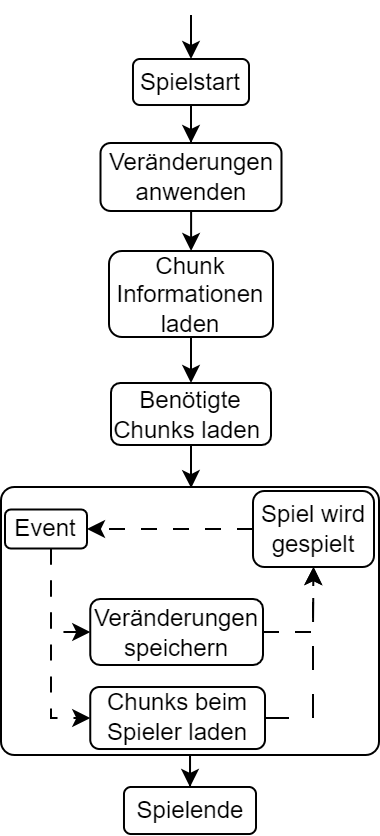
\includegraphics[width=0.36\textwidth]{images/Chunkbasiert2.png}
    \caption{Alternative zu dem Chunk-basierten System}
    \label{fig:altchunkBasedSystem}
\end{figure}

\begin{figure}[htp]
    \centering
    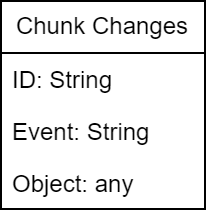
\includegraphics[width=0.25\textwidth]{images/Changes.png}
    \caption{Speichern von Veränderungen}
    \label{fig:changesClass}
\end{figure}

\begin{itemize}
    \item Veränderungen anwenden:
    \begin{itemize}
        \item Liste von Veränderungen des letzten Spielstandes werden lokal gespeichert (zum Beispiel als Objekte wie \ref{fig:changesClass} in JSON)
        \item Verschiedene Events = Unterschiedlich was Object ist
        \item Liste von oben nach unten abarbeiten, da erste Einträge die ältesten sind 
        \item Objekte aus Liste zu Chunk hinzufügen/updaten oder (bei dynamischer Chunkgröße) Chunks die nicht mehr gebraucht werden löschen
        \item Liste leeren
    \end{itemize}
    \item Nearby loading von Chunks wie beim anderen Chunk-basierten System
    \item Chunk-Veränderung speichern:
    \begin{itemize}
        \item Hinzugefügte/Veränderte/Gelöschte Objekte in Change Liste (im Arbeitsspeicher) speichern
        \item Entweder direkt in lokaler Change List Datei ans Ende hinzufügen oder erst bei Spielende (sehr riskant, falls Spiel ungewollt terminiert)
        \item Bei dynamischer Chunkgröße speichern wenn Chunks gelöscht/hinzugefügt wurden
    \end{itemize}
\end{itemize}
%--------------------------------------------------------------------------


%--------------------------------------------------------------------------
\subsection{Auswertung}
Auswertung der Strategien mit Daten/einfaches Spielkonzept mit Java und JSON testen:
\begin{itemize}
    \item Spieler (HP, LVL, Ausrüstung, Position, Rotation, ...)
    \item Gegner (HP, LVL, Ausrüstung, Position, Rotation, ...)
    \item Ausrüstung (Beschreibung/ID, Verteidigung, Angriff)
    \item Hindernisse (Beschreibung/ID, Position, Rotation)
    \item Items (Beschreibung/ID, Position, Rotation)
\end{itemize}

\begin{figure}[htp]
    \centering
    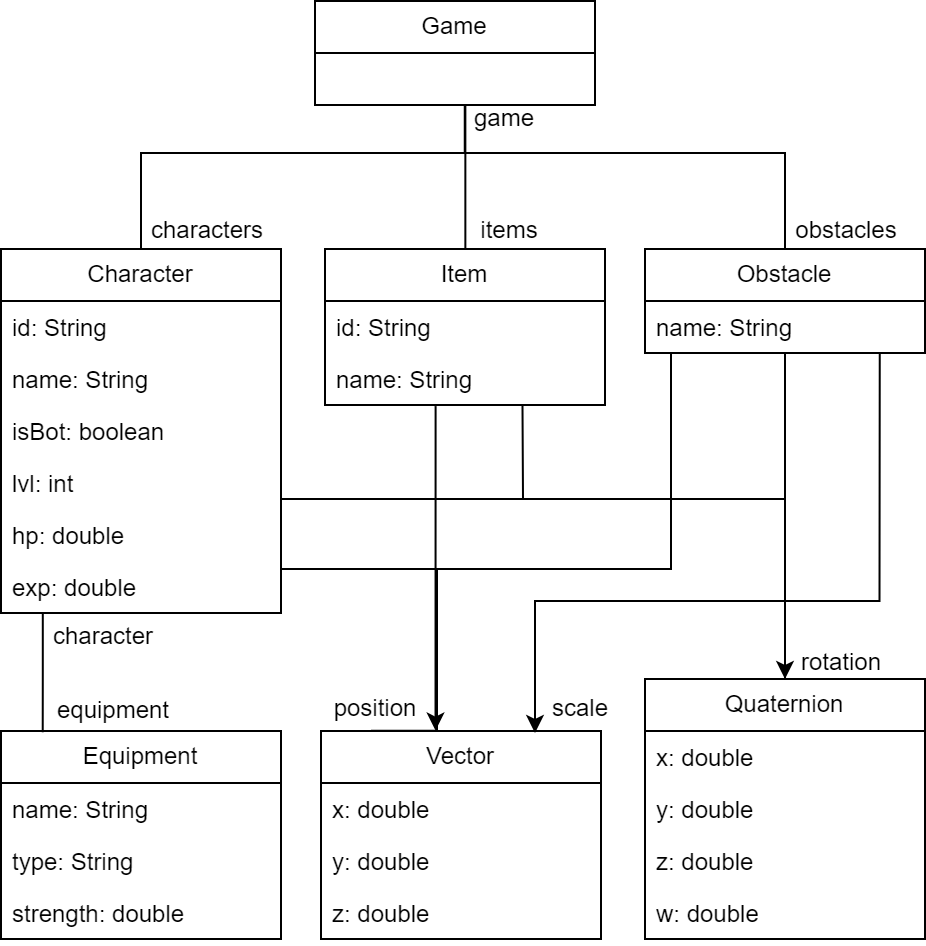
\includegraphics[width=0.8\textwidth]{images/Klassendiagramm.png}
    \caption{Klassendiagramm des Spieles}
    \label{fig:classDia}
\end{figure}

Klassendiagramm zeigen, um Daten des Spieles zu visualisieren. Testen der Effizienz mit JMH (Erklären was JMH ist und warum das gut dafür ist)

Zu beachtende Faktoren:
\begin{itemize}
    \item Chunk size
    \item Veränderungen
\end{itemize}